\documentclass[10pt,letterpaper]{article}
%\usepackage{times}
\usepackage[margin=1in,hmargin=1in]{geometry}
\usepackage{amsmath}
\usepackage{tikz,url}
\usepackage{amssymb}
\usepackage{fancyhdr}
\usetikzlibrary{matrix}
\usepackage{listings}
\usepackage{tabularx}
\usepackage{xcolor}
\usepackage{graphicx}
\usepackage{graphics}
\usepackage{titling}
\pagestyle{fancy}
\usepackage{float}
\usepackage{fancyvrb}
\usepackage{verbatim}
\usepackage{enumitem}
\usepackage{alltt}
\usepackage{pdfpages}
%\usepackage{float}
%\restylefloat{table}

\fancyhead[LO]{STAT W4201 Advanced Data Analysis}
\fancyhead[RO]{HW 2}
\fancyhead[LE]{STAT W4201 Advanced Data Analysis}
\fancyhead[RE]{HW 2}
\title{\textbf {Homework 2}}
\author{{Qianbo Wang}\\{uni: qw2180}}
\date{}
\setlength{\droptitle}{-5em}
\setlength{\parindent}{0pt}
\makeatletter
\newcommand{\rmnum}[1]{\romannumeral #1}
\newcommand{\Rmnum}[1]{\expandafter\@slowromancap\romannumeral #1@}
\makeatother
\lstset{
language=R,
tabsize=4, 
%frame=shadowbox, 
commentstyle=\color{red!50!green!50!blue!50},
%rulesepcolor=\color{red!20!green!20!blue!20},
keywordstyle=\color{blue!90},
showstringspaces=false,
stringstyle=\ttfamily, 
keepspaces=true, 
breakindent=22pt, 
numbers=none,
stepnumber=1,
numberstyle=\tiny, 
numberstyle={\color[RGB]{0,192,192}\tiny} ,
numbersep=5pt,  
basicstyle=\footnotesize, 
showspaces=false, 
flexiblecolumns=true, 
comment=[l]{\#},
texcl=true,
escapeinside={\$$}{\^^M},
breaklines=true, 
breakautoindent=true,
breakindent=4em, 
aboveskip=1em, 
tabsize=2,
showstringspaces=false, 
backgroundcolor=\color[RGB]{244,244,244},   
fontadjust,
captionpos=t,
framextopmargin=2pt,framexbottommargin=2pt,abovecaptionskip=-3pt,belowcaptionskip=3pt,
extendedchars=false,columns=flexible
}

\begin{document}
\maketitle
\thispagestyle{fancy}
\vspace{-2em}

\textbf{Consider the crabs data frame in R library MASS which has 200 rows and 8 columns, describing 5 morphological measurements on 50 crabs each of two color forms ("B" or "O" for blue or orange) and both sexes, of the species Leptograpsus variegatus collected at Fremantle, W. Australia. data(crabs, package="MASS")}
\section*{Problem 1}
\textbf{Determine whether there is a significant difference between blue and orange crabs in mean carapace length (mm) [CL] using each of the following procedures:}
\begin{enumerate}[leftmargin=0cm,itemindent=.5cm,labelwidth=\itemindent,labelsep=0cm,align=left]
\item[\textbullet] \textbf{A parametric procedure}

Since this test compares the means of two groups, then we should use two sample T-test. And the null and alternative hypothesis are:
$$H_0: \mu_B=\mu_O ~~and~~H_1: \mu_B\neq \mu_O$$
The result is as follows:
\begin{center}
Two Sample T-test Result
\verbatiminput{ttest1.txt}
\end{center}
Since the $p-value=3.468*10^{-5}<0.05$. Then we should reject the null, which means that there is a significant difference between blue and orange crabs in mean carapace length. 

\item[\textbullet] \textbf{A nonparametric procedure}

Since this test compares the means of two groups, then we should use Wilcoxon rank sum test. Still the null and alternative hypothesis are:
\[H_0: \mu_B-\mu_O=0 ~~and~~H_1: \mu_B-\mu_O\neq 0\]
And the result is as follows:
\begin{center}
Wilcoxon Rank Sum Test Result
\verbatiminput{wilcoxtest1.txt}
\end{center}
Since the $p-value=7.469*10^{-5}<0.05$. Then we should reject the null, which means that there is a significant difference between blue and orange crabs in mean carapace length. 

\item[\textbullet] \textbf{A resampling procedure}

Since this test compares the means of two groups, then we can use bootstrap method to resample. And use bootstrap test procedure. Still the null and alternative hypothesis are:
\[H_0: \mu_B-\mu_O=0 ~~and~~H_1: \mu_B-\mu_O\neq 0\]
Since the $p-value=0<0.05$ we should reject the null, which means that there is a significant difference between blue and orange crabs in mean carapace length. 
\end{enumerate}

\section*{Problem 2}
\textbf{Discuss the assumptions underlying the analyses in Problem 1 above, their validity, and any remedial measures to be taken.}
\begin{enumerate}[leftmargin=0cm,itemindent=.5cm,labelwidth=\itemindent,labelsep=0cm,align=left]
\item[\textbullet] \textbf{Parametric Test}

In T Test, it assumes that the two groups data satisfy i.i.d. normal distribution. \\
First, check if there exist outlier. Draw the box plot to check.
\begin{center}
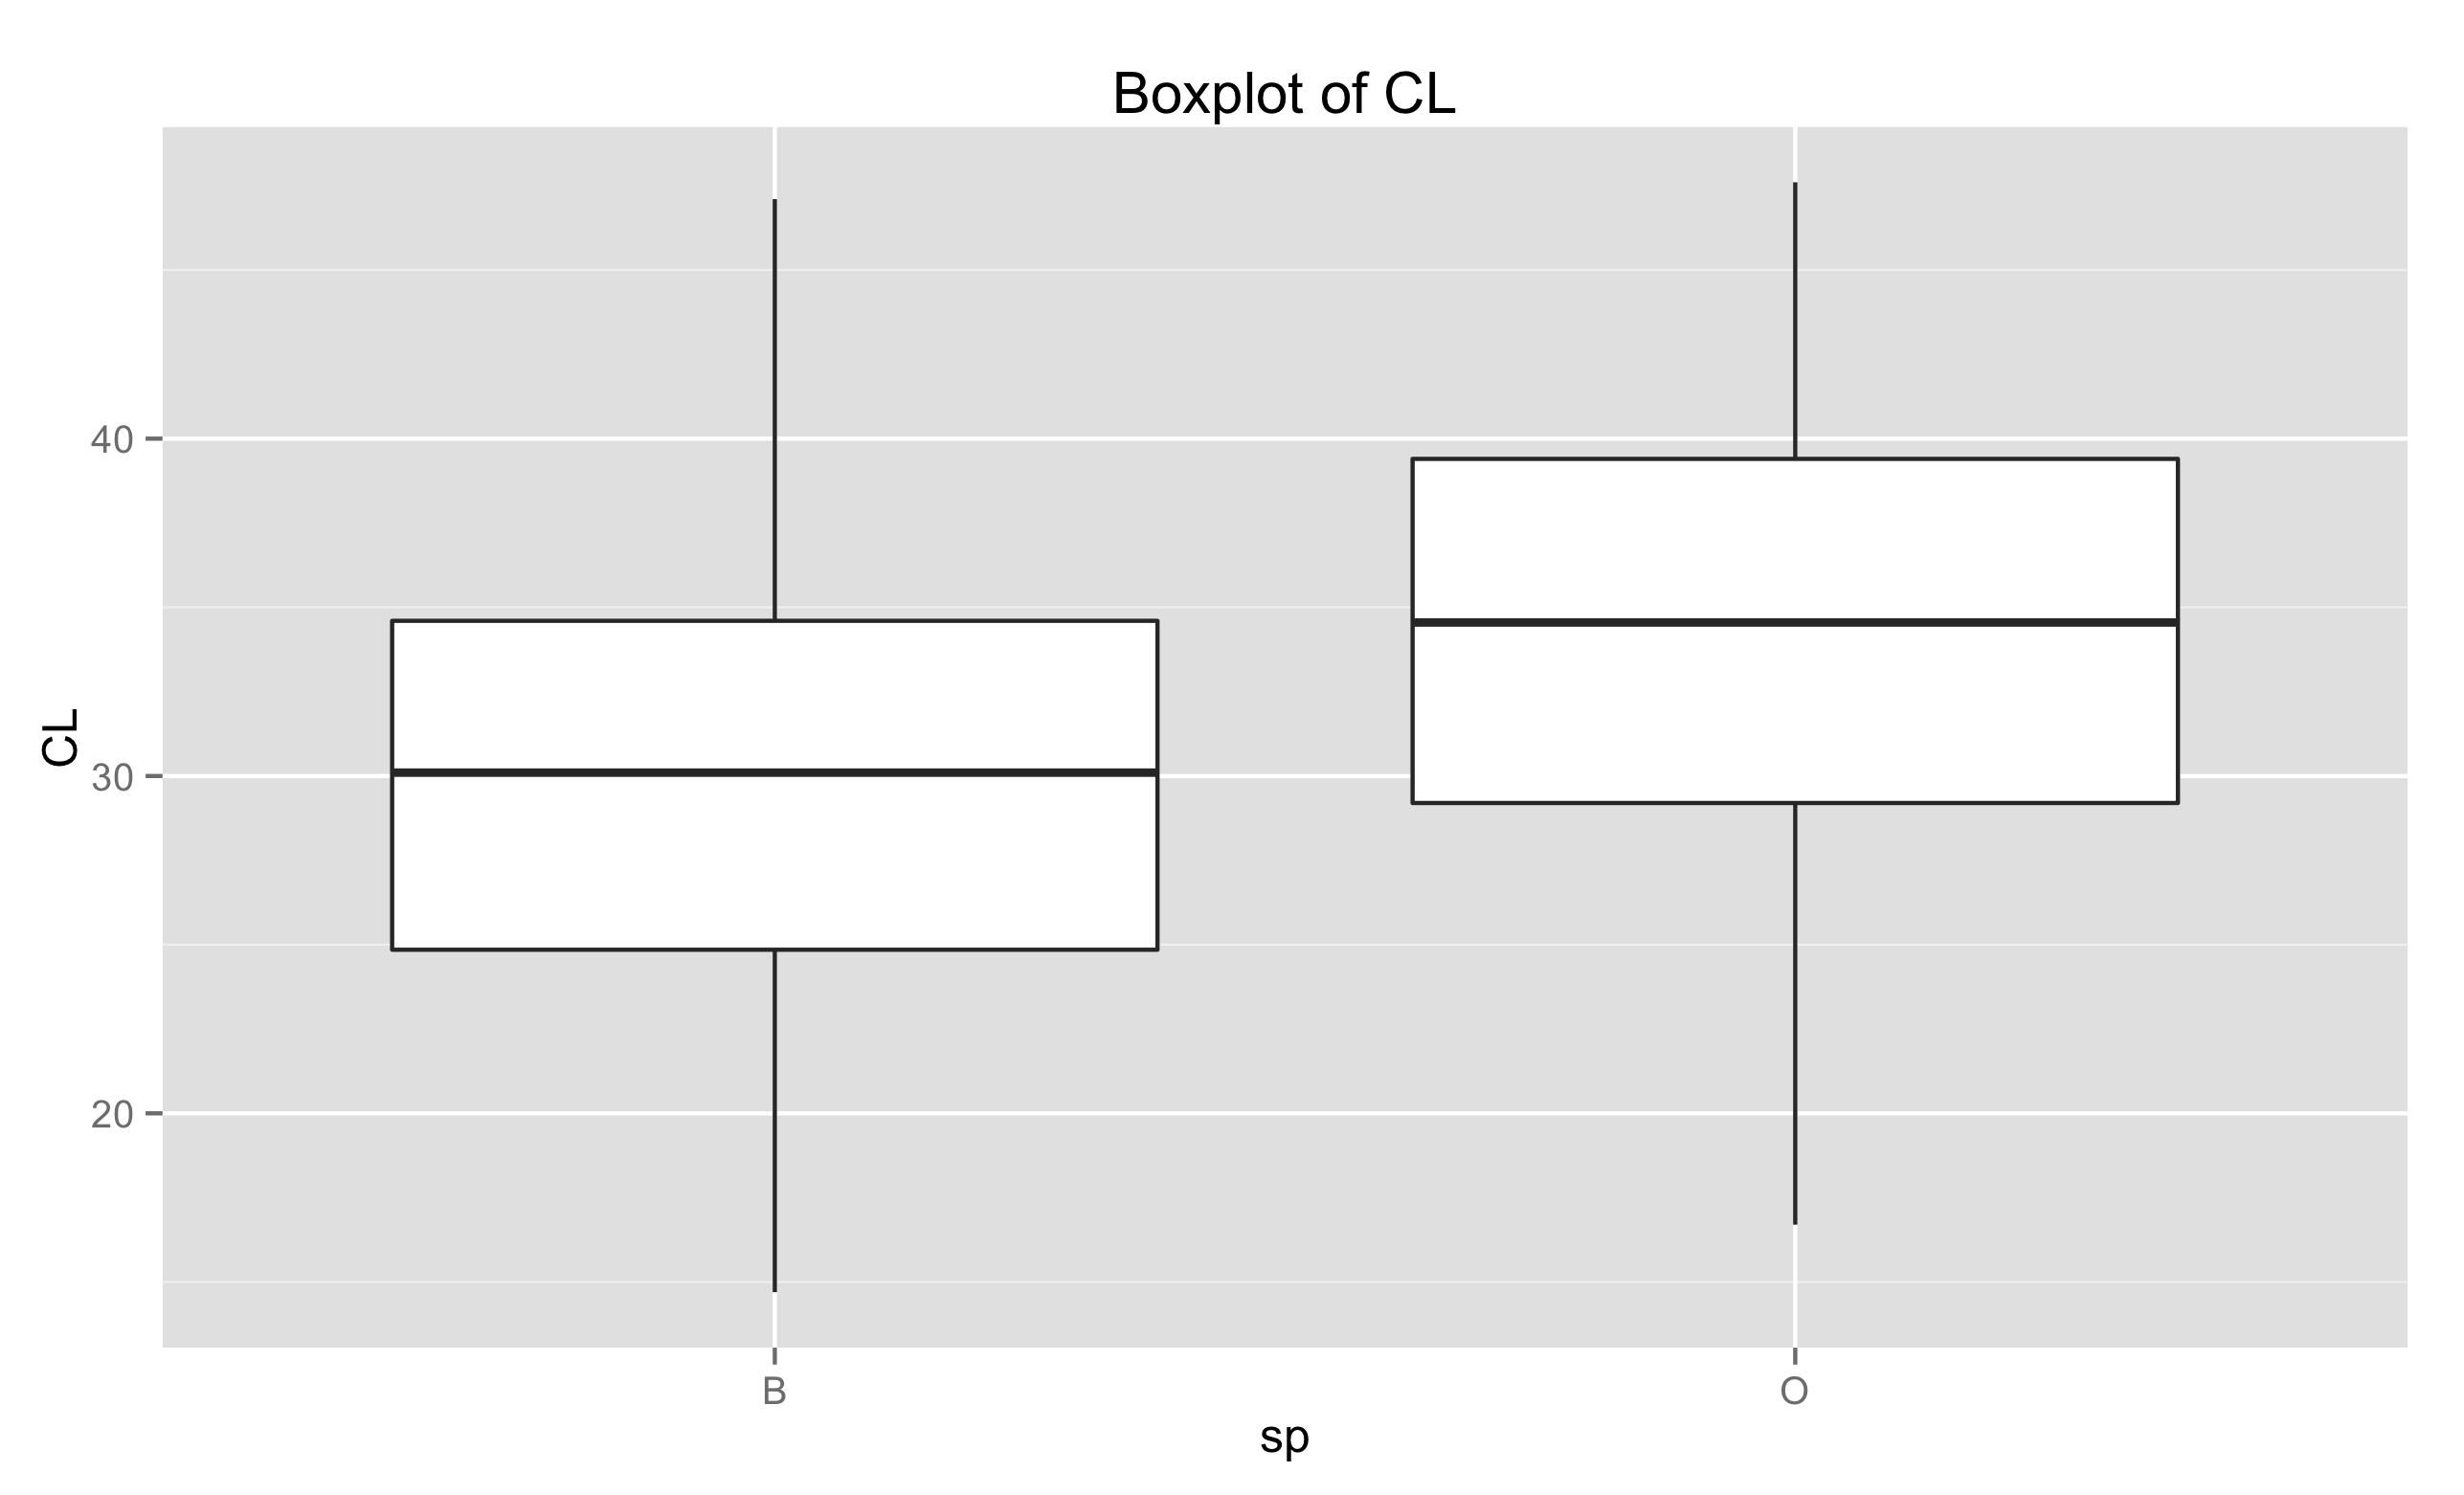
\includegraphics[scale=0.13]{boxgroup}
\end{center}
Second, check the assumptions in normality. Draw Q-Q plot to check. 
\begin{center}
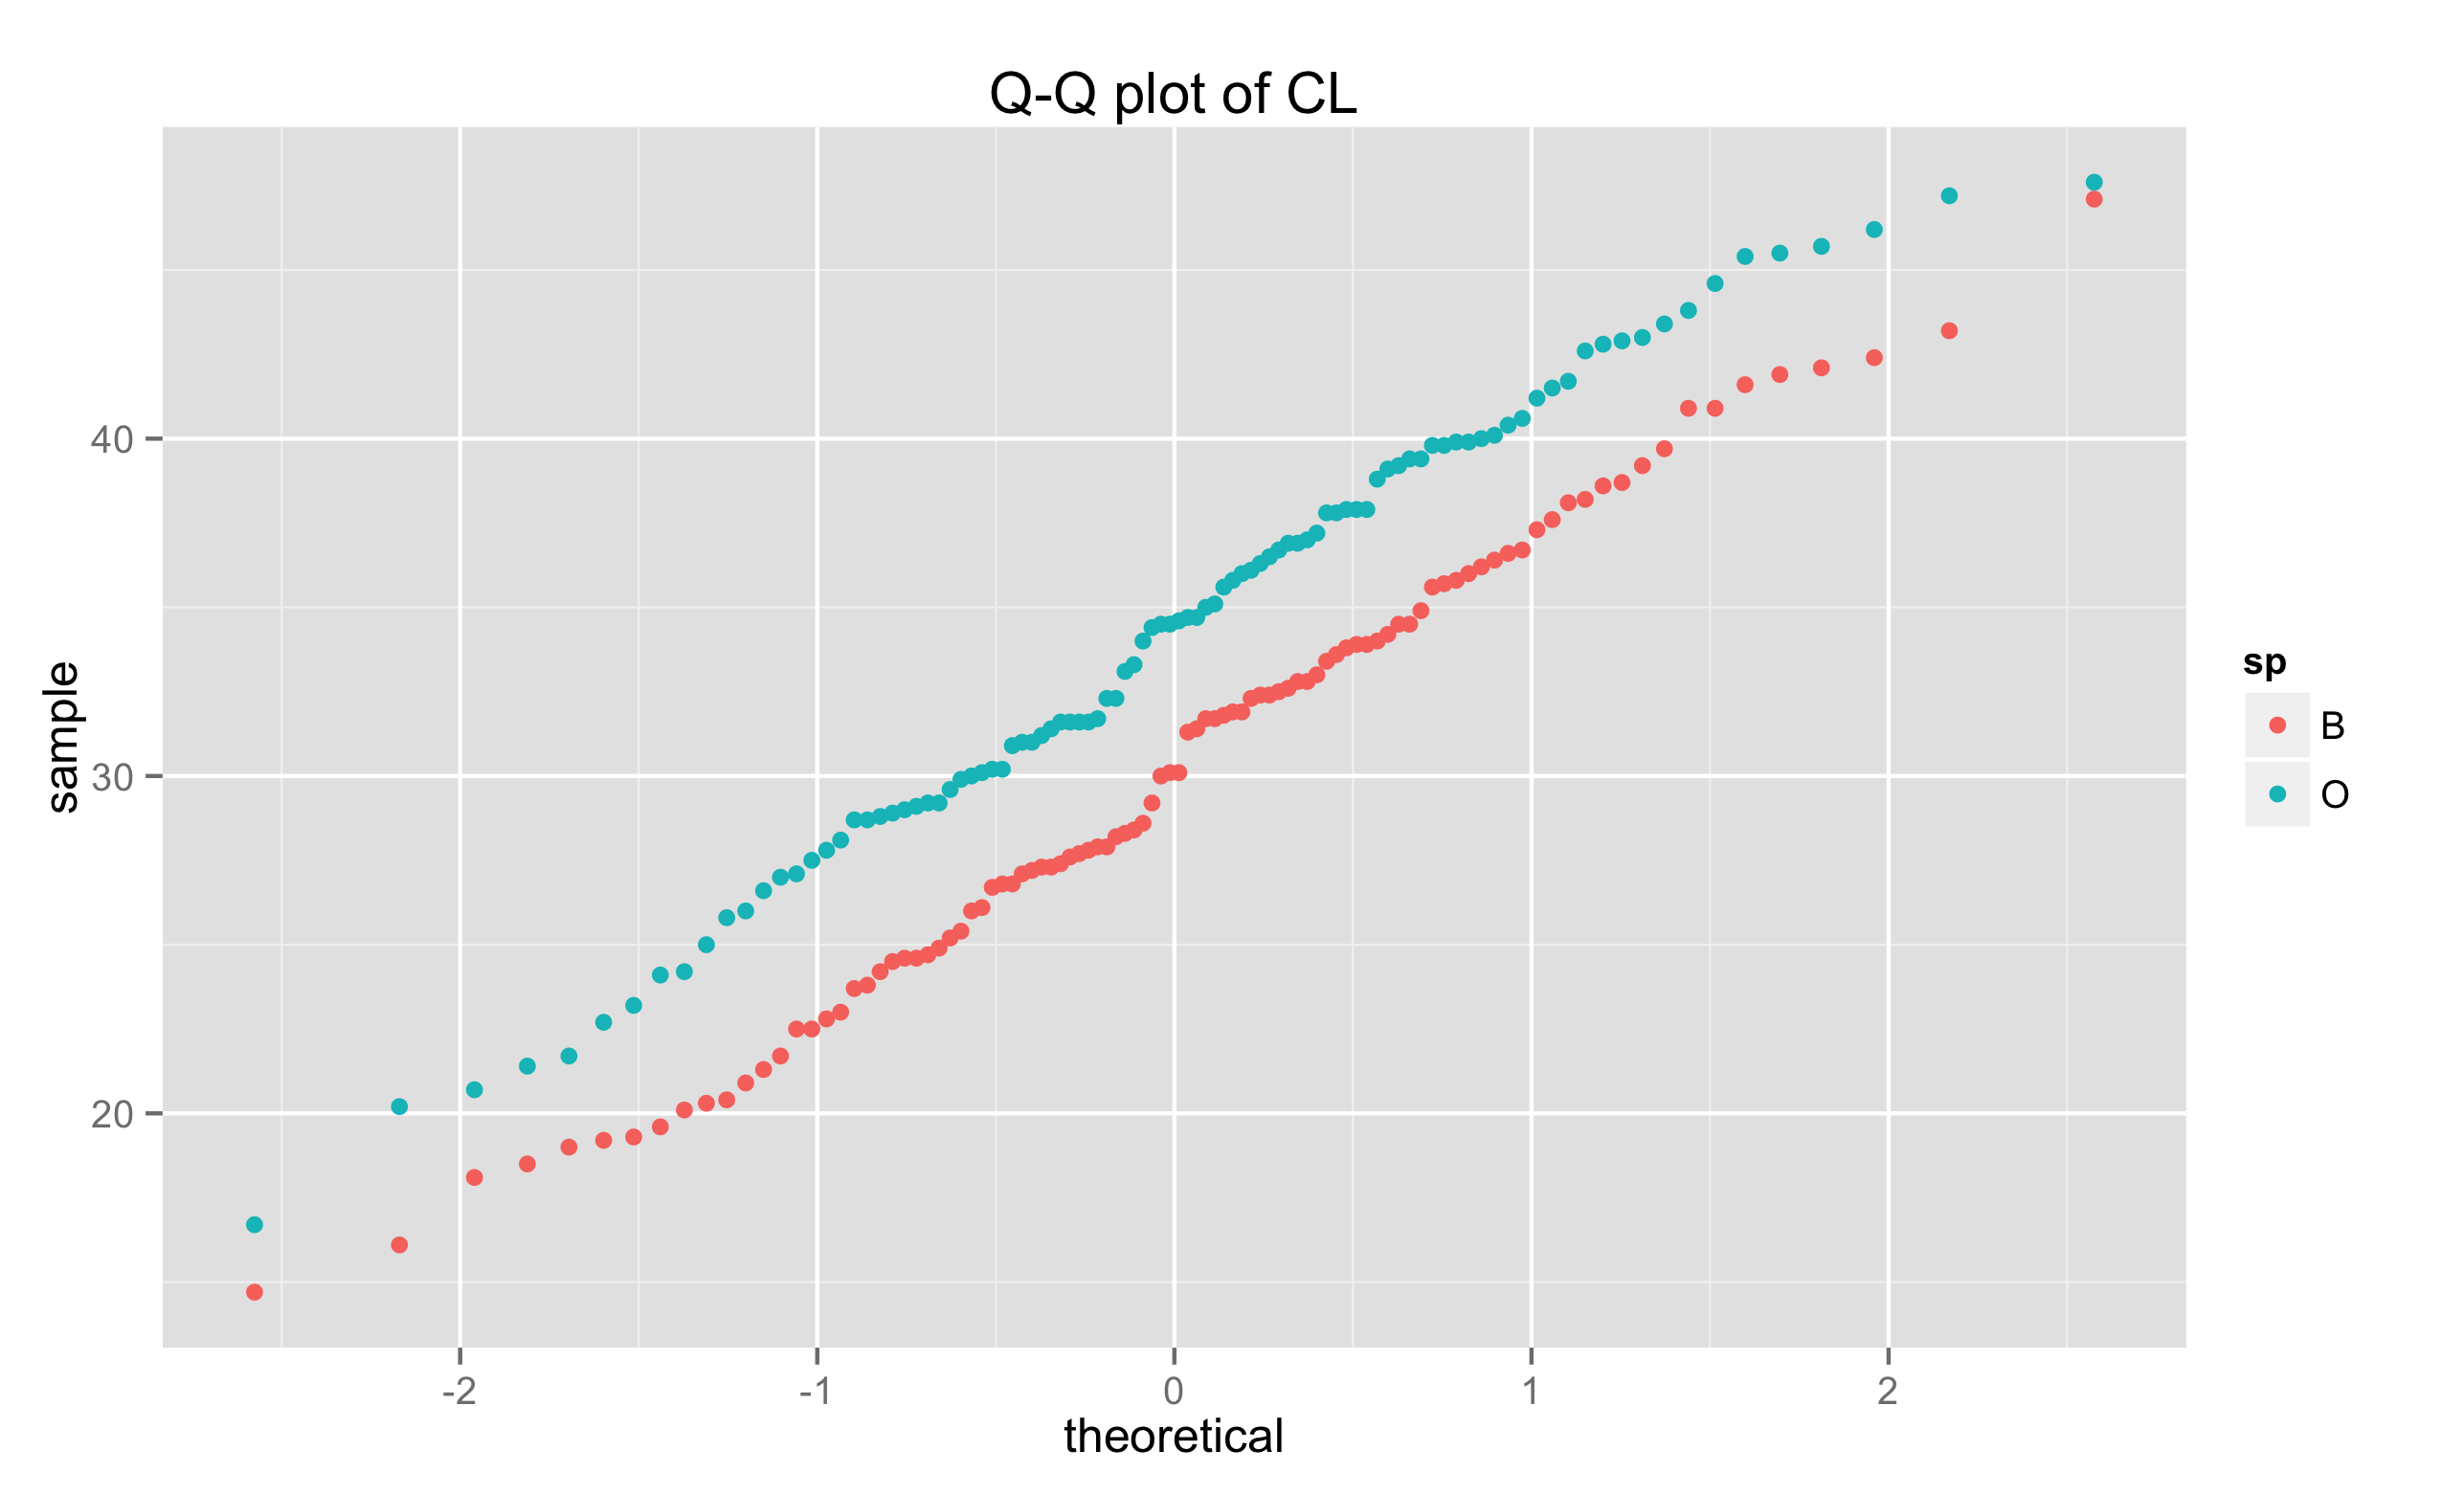
\includegraphics[scale=0.13]{qqplot}
\end{center}
I use shapiro test to test the normality. The results are as follows:
\begin{center}
Shapiro Test Result
\verbatiminput{normaltest.txt}
\end{center}
 
Since the p-value for the Blue Group is $p-value=0.6745$, and the p-value for the Orange Group is $p-value=0.5557$, so we can not reject the null hypothesis for both groups. Then we can conclude that the data are approximately normal distributed.\\
Then, check the skewness and kurtosis, the skewness of the two groups are $S_B=0.02571518$ and $S_O=-0.1536776$. The excess kurtosis of the two groups are $K_B=-0.651835$ and $K_O=-0.5626413$, since both skewness and kurtosis of two groups are close to each other and close to 0. Then the normality are approximately valid.\\
Then check the independence of the two variables, use correlation test, the result is as follows:
\begin{center}
Correlation Test Result
\verbatiminput{cortest.txt}
\end{center}
Since the crabs were captured in the same place then it could not be dependent. And use correlation test, since the p-value is $p-value=2.2*10^{-16}$, then we should reject the null, which means Orange and Blue are not independent.\\
Since there is no outlier and the data are approximately normal distributed, then the assumptions of i.i.d. normal distributed is approximately valid.\\
About Remedial measures to be taken, I think we can take log of the data, since the data are not so well normal distributed. If take the log, then the data can be more close to normal distributed and independent.
\item[\textbullet] \textbf{Nonparametric Test}

In Wilcoxon Rank Sum Test, since the data size is 100, which is large enough.Then it only assumes that the data from two groups is independent. From the first part's conclusion,  we can assume  independence 
\item[\textbullet] \textbf{Resampling Test}

In Bootstrap Method, since the data size is 100, it assumes that each sub sampling is independent and identical distribution. In other words, it assumes that the sub samples come from the same distribution of then population, but each sample is drawn independently from the other samples. And since we use with replacement method, we just use the empirical distribution to estimate the population. \\
\end{enumerate}

\section*{Problem 3}
\textbf{Ramsey and Schafer (2nd ed., p. 576), Data Problem 17 (Alcohol Consumption and Breast Cancer)}
\begin{enumerate}[leftmargin=0cm,itemindent=.5cm,labelwidth=\itemindent,labelsep=0cm,align=left]
\item[\textbullet] In the group of $<21kg/m^2$

First, calculate the excess, there is an excess of $5.4576$ heavy drinkers. Second, calculate the variance, $variance= 10.26978$. Third, calculate the z-statistic, $z=1.703034$. Then, calculate the p-value, $p-value=0.04428083$.\\

\item[\textbullet] In the group of $21-25kg/m^2$

First, calculate the excess, there is a negative excess of $-8.437908$ heavy drinkers. Second, calculate the variance, $variance = 25.88573$. Third, calculate the z-statistic, $z=-1.658459$. Then, calculate the p-value, $p-value=0.9513875$.\\

\item[\textbullet] In the group of $>25kg/m^2$

First, calculate the excess, there is an excess of $3.078261$ heavy drinkers. Second, calculate the variance, $variance = 12.51782$. Third, calculate the z-statistic, $z=0.8700438$. Then, calculate the p-value, $p-value=0.1921382$.
 \end{enumerate}
Overall, there is a 0.09797949 excess heavy drinkers among cases. And for the group of $<21kg/m^2$, the odds ratio is $1.714497$ with 
 $95\%$ confidence interval $= [1.055654 , 2.536338]$, and for the group of $21-25kg/m^2$, the odds ratio is $0.7197134$ with 
 $95\%$ confidence interval $= [0.4878431 , 1.0617909]$, and for the group of $>25kg/m^2$, the odds ratio is $1.30102$ with 
 $95\%$ confidence interval $= [0.735191 , 2.302332]$\\

Since the Mantel-Haenszel test works well when the relative odds are the same in the sub-tables. So we can not use Mantel-Haenszel test for the overall 3 tables. We can compare odds ratio for 3 individual tables.\\
So there is evidence that the odds ratios are different. Thus, the tables should be summarized separately in 3 different groups. And for the group of $<21kg/m^2$, the odds ratio is $1.714497$ ,which means heavy drinkers are 1.055654 to 2.536338 times light drinkers on risk of cancer, with 
 $95\%$ confidence interval $= [1.055654 , 2.536338]$, and for the group of $21-25kg/m^2$, the odds ratio is $0.7197134$, ,which means heavy drinkers are 0.4878431 to 1.0617909 times light drinkers on risk of cancer,with $95\%$ confidence interval $= [0.4878431 , 1.0617909]$, and for the group of $>25kg/m^2$, the odds ratio is $1.30102$, which means heavy drinkers are 0.735191 to 2.302332 times light drinkers on risk of cancer, with  $95\%$ confidence interval $= [0.735191 , 2.302332]$.\\

\textbf{Conclusion: Since the odds ratio are different in 3 groups. The data are consistent with the proposition that heavy drinking is associated with higher risk of breast cancer among large body mass women and small body mass women but not among women with body mass about $21-25 kg/m^2$.}

\section*{Problem 4}
\textbf{Ramsey and Schafer (2nd ed., p. 550), Data Problem 18 (Hale-Bopp and Handedness)}\\

Since we want to check if there is association between left or right handedness and correct recollection. Then use Proportion Test, which compare and test the odds of the two groups. The null and alternative hypothesis are:
\[H_0: odds \ ratio=0 ~~and~~H_1: odds \ ratio\neq 0 \] 
First, calcualte the log odds for the two groups. The log odds is $0.4924406$.\\
Second, calculate the proportion from the combined sample. $\pi_c=0.7055838$.\\
Third, calculate SE for the log odds ratio estimate. ${SE}_0=0.2210684$.\\
Then, calculate z-statistic, $z=2.227548$, and $p-value=0.01295532$.\\
Finally, calculate the $95\%$ confidence interval of the log odds, $95\%$ CI $= [0.05416004 , 0.93072115]$, and $95\%$ confidence interval of the odds ratio, which is $95\%$ CI $= [1.055654 , 2.536338]$.\\

\textbf{Conclusion: Since the p-value is 0.0129, which means that we should reject the null hypothesis, i.e. the odds ratio is not 1 in two groups.  So we can conclude that, the data indicate that left- or right-handedness is associated with correct recollection of the orientation. \\
And the $95\%$ confidence interval for the difference of the proportion is $[1.055654 , 2.536338]$, which means that the odds
of a correct answer for a right handed person are approximately $1.636305$ times that for a right handed person with $95\%$ CI $[1.055654 , 2.536338]$. }


\newpage
\noindent {\textbf{R Code}:}
\begin{lstlisting}
#Problem 1
library(MASS)
Blue<-crabs$CL[crabs$sp=="B"]
Orange<-crabs$CL[crabs$sp=="O"]

#t test
t.test(Blue,Orange)
sink("/Users/raymond/Desktop/STAT W4201/HW2/ttest1.txt")
t.test(Blue,Orange)
sink()

#wilcoxon rank sum test
wilcox.test(Blue,Orange)
sink("/Users/raymond/Desktop/STAT W4201/HW2/wilcoxtest1.txt")
wilcox.test(Blue,Orange)
sink()

#bootstrap test
zObs<-(mean(Blue)-mean(Orange))/sqrt(var(Blue)/length(Blue)+var(Orange)/length(Orange))
OrangeNew<-Orange+mean(Blue)-mean(Orange)
set.seed(123)
zSam<-rep(NA,1000)
for(i in 1:1000){
  BlueSam<-sample(Blue,length(Blue),replace=T)
  OrangeSam<-sample(OrangeNew,length(OrangeNew),replace=T)
  zSam[i]<-(mean(BlueSam)-mean(OrangeSam))/sqrt(var(BlueSam)/length(BlueSam)+var(OrangeSam)/length(OrangeSam))
}
pValue<-sum(abs(zSam)>=abs(zObs))/length(zSam)

#Problem 2
#qqplot check normality assumption
library(ggplot2)
qqplot<-ggplot(crabs,aes(sample=CL))
qqplot+stat_qq(aes(color=sp))+ggtitle("Q-Q plot of CL")
ggsave(file="/Users/raymond/Desktop/STAT W4201/HW2/qqplot.png")

#boxplot check outliers
box<-ggplot(crabs,aes(sp,CL))
box+geom_boxplot()+ggtitle("Boxplot of CL")
ggsave(file="/Users/raymond/Desktop/STAT W4201/HW2/boxgroup.png")

#test normality
shapiro.test(Blue)
shapiro.test(Orange)
sink("/Users/raymond/Desktop/STAT W4201/HW2/normaltest.txt")
shapiro.test(Blue)
shapiro.test(Orange)
sink()


#check skewness
library(e1071)
s1<-skewness(Blue)
s2<-skewness(Orange)
k1<-kurtosis(Blue)
k2<-kurtosis(Orange)
#Problem 3
#in <21 group
expected1<-90*64/177
excess1<-38-90*64/177
var1<-90*87*64*113/(177*177*176)
zstat1<-excess1/sqrt(var1)
pValue1<-1-pnorm(zstat1)

#in 21-25 group
expected2<-212*159/459
excess2<-65-212*159/459
var2<-212*247*159*300/(459*459*458)
zstat2<-excess2/sqrt(var2)
pValue2<-1-pnorm(zstat2)

#in >25 group
excess3<-30-72*86/230
var3<-72*158*86*155/(230*230*229)
zstat3<-excess3/sqrt(var3)
pValue3<-1-pnorm(zstat3)
#calculate total excess
excesstot<-excess1+excess2+excess3
vartot<-var1+var2+var3
zstattot<-excesstot/sqrt(vartot)

#calculate odds in <21 group
odds_g1<-38*61/(52*26)
pic_g1<-(38+61)/177
se0_g1<-sqrt(1/(90*pic_g1*(1-pic_g1))+1/(87*pic_g1*(1-pic_g1)))
se_g1<-sqrt(1/38+1/52+1/26+1/61)
zstat_g1<-log(odds_g1)/se0_g1
pValue_g1<-1-pnorm(zstat_g1)
CI_g1<-exp(log(odds_g1)+1.96*c(-se_g1,se_g1))

#calculate odds in 21-25 group
odds_g2<-65*153/(147*94)
pic_g2<-(65+153)/459
se0_g2<-sqrt(1/(212*pic_g2*(1-pic_g2))+1/(247*pic_g2*(1-pic_g2)))
se_g2<-sqrt(1/65+1/147+1/94+1/153)
zstat_g2<-log(odds_g2)/se0_g2
pValue_g2<-1-pnorm(zstat_g2)
CI_g2<-exp(log(odds_g2)+1.96*c(-se_g2,se_g2))

#calculate odds in >25 group
odds_g3<-30*102/(42*56)
pic_g3<-(30+102)/230
se0_g3<-sqrt(1/(72*pic_g3*(1-pic_g3))+1/(158*pic_g3*(1-pic_g3)))
se_g3<-sqrt(1/30+1/42+1/56+1/102)
zstat_g3<-log(odds_g3)/se0_g3
pValue_g3<-1-pnorm(zstat_g3)
CI_g3<-exp(log(odds_g3)+1.96*c(-se_g3,se_g3))

#Problem 4
logodds<-log(149*68/(129*48))
pic<-(149+129)/(197+197)
se0<-sqrt(1/(197*pic*(1-pic))+1/(197*pic*(1-pic)))
se<-sqrt(1/149+1/129+1/48+1/68)
zstat<-logodds/se0
pValue<-1-pnorm(zstat)
CI<-logodds+1.96*c(-se,se)

\end{lstlisting}
\end{document}